% !TeX spellcheck = en_US
\documentclass[hidelinks,titlepage,a4paper]{article}

\usepackage[utf8]{inputenc}
\usepackage[T1]{fontenc}
\usepackage{lmodern}
\usepackage{newpxtext,newpxmath}
\linespread{1.05} % Line spacing - Palatino needs more space between lines
\usepackage{microtype}
\usepackage[group-separator={,}]{siunitx}
\usepackage[tikz]{bclogo}
\usepackage{pgfplots}
\usepackage{appendix}
\usepackage{verbatim}
\usepackage[hyphens]{url}
\usepackage{hyperref} % For hyperlinks in the PDF
\usepackage{fontawesome5}
\usepackage[os=win]{menukeys}

\usepackage[hmarginratio=1:1,top=32mm,columnsep=20pt]{geometry} % Document margins
\geometry{a4paper,textwidth=6.5in,hmarginratio=1:1,
  textheight=9in,vmarginratio=1:1,heightrounded}

\usepackage{titlesec}
\setcounter{secnumdepth}{4}
\setcounter{tocdepth}{4}

\titleformat{\paragraph}
{\normalfont\normalsize\bfseries}{\theparagraph}{1em}{}
\titlespacing*{\paragraph}
{0pt}{3.25ex plus 1ex minus .2ex}{1.5ex plus .2ex}

\usepackage{fancyhdr} % Headers and footers
\pagestyle{fancy} % All pages have headers and footers
\fancyhead{} % Blank out the default header
\fancyfoot{} % Blank out the default footer
\fancyhead[L]{Tracy Profiler}
\fancyhead[R]{Technical documentation}
\fancyfoot[RO]{\thepage} % Custom footer text

\usepackage{listings}
\usepackage{xcolor}
\usepackage{float}
\lstset{language=C++}
\lstset{
         basicstyle=\footnotesize\ttfamily,
         tabsize=4,
         extendedchars=true,
         breaklines=true,
         stringstyle=\ttfamily,
         showspaces=false,
         xleftmargin=17pt,
         framexleftmargin=17pt,
         framexrightmargin=5pt,
         framexbottommargin=4pt,
         showstringspaces=false,
         escapeinside={@}{@},
         aboveskip=\baselineskip,
         belowskip=\baselineskip
}

\usepackage[hang, small,labelfont=bf,up,textfont=it,up]{caption} % Custom captions under/above floats in tables or figures

\usepackage{tikz}
\usetikzlibrary{arrows.meta,positioning,shapes,patterns}

\newcommand{\LMB}{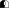
\includegraphics[height=.8\baselineskip]{icons/lmb}}
\newcommand{\RMB}{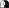
\includegraphics[height=.8\baselineskip]{icons/rmb}}
\newcommand{\MMB}{
\includegraphics[height=.8\baselineskip]{icons/mmb}}
\newcommand{\Scroll}{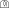
\includegraphics[height=.8\baselineskip]{icons/scroll}}

\newcommand*\circled[1]{\tikz[baseline=(char.base)]{
    \node[shape=circle,draw,inner sep=1.5pt] (char) {#1};}}

\begin{document}

\begin{titlepage}
\centering
{\fontsize{120}{140}\selectfont Tracy Profiler}

\vspace{50pt} {\Huge\fontfamily{lmtt}\selectfont Technical documentation}

\vfill 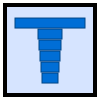
\includegraphics[height=40mm]{../icon/icon}

\vfill
\large\textbf{Bartosz Taudul} \href{mailto:wolf.pld@gmail.com}{<wolf.pld@gmail.com>}

\vspace{10pt}
\today
\vfill
\url{https://bitbucket.org/wolfpld/tracy}
\end{titlepage}

\begin{abstract}
This is the technical documentation of the Tracy Profiler. It is meant as a guide for developers who want to learn how Tracy works in detail, add new features, or fix bugs. If you only want to use the profiler in your application, you will not find anything of interest here and you should instead read \emph{The user manual}, which describes how the profiler can be used.

This document assumes that you have basic knowledge of how the Tracy Profiler works, as the concepts which are already described in the user manual won't be covered here.

The information found in this documentation is intended to give you only a brief overview of the algorithms and data structures used in the profiler. It may be incomplete, cursory, or even plainly wrong. This is not a requirements specification. As usual, the source code is the ultimate place to gain knowledge and insight. You are expected to do your homework.
\end{abstract}

\tableofcontents

\newpage

\section{Source repository structure}

Tracy Profiler is split into the following parts:

\begin{itemize}
\item Source files in the root directory -- public interface to used by the profiled applications. Part of the client.
\item \emph{client} directory -- private source files specific to the client part of the profiler.
\item \emph{common} directory -- private source files shared by both the client and server parts.
\item \emph{server} directory -- private source files specific to the server part of the profiler.
\item End user applications
\begin{itemize}
\item \emph{capture} directory -- command line server interface.
\item \emph{profiler} directory -- GUI server interface.
\item \emph{update} directory -- server wrapper which loads and then saves the trace file.
\end{itemize}
\item \emph{test} directory -- command line program used to test client integration.
\item \emph{doc}, \emph{icon}, \emph{manual} directories -- documentation and image assets.
\item \emph{imgui}, \emph{imguicolortextedit}, \emph{libbacktrace}, \emph{nfd} directories -- external libraries used by the profiler.
\end{itemize}

\section{Build process}

End user applications are using MSVC as a base for development. The project files are located in the \texttt{build/win32} directory. Unix build system, located in the \texttt{build/unix} directory is extracting source file list from the MSVC solution and optionally can filter-out some source files or add another. Refer to the build scripts of \texttt{profiler} utility for an example.

\subsection{Unix details}

A makefile based system is used. The main \texttt{Makefile} is used only to dispatch the build, supporting the following targets:

\begin{itemize}
\item \texttt{debug} (default)
\item \texttt{release}
\item \texttt{clean}
\end{itemize}

The \texttt{debug.mk} and \texttt{release.mk} files only set a few of the optimization related variables and include the main \texttt{build.mk} file.

In the header of the \texttt{build.mk} file you can find definitions of the resulting executable name, list of used libraries, required include paths, etc. Most of the file is boilerplate required to extract build dependencies, or pass the appropriate flags to compiler and linker.

\section{Client part}

The client portion of Tracy is basically a queue. Application threads are producing queue items through the instrumentation macros and a dedicated profiler thread consumes the items to send them over the network, to the server.

Tracy functions, libraries, data structures are contained in the \texttt{tracy} namespace.

\subsection{Memory resources}

Tracy uses the \emph{rpmalloc} allocator to completely separate itself from the heap used by the application. Rpmalloc is wrapped by the \texttt{tracy\_malloc()} and \texttt{tracy\_free()} functions, found in the \texttt{common/TracyAlloc.hpp} header file.

\subsection{Timer queries}
\label{timerqueries}

Current time may be obtained by calling the \texttt{GetTime()} function.

Tracy tries to achieve maximum possible timer resolution, to make measurements as accurate as possible. This is done in the following ways:

\begin{itemize}
\item On x86/x64 an assembly instruction \texttt{rdtscp} is always used to obtain the raw hardware timer reading. Systems with the \texttt{TSD} (Time Stamp Disable) flag set are not supported.
\item On ARM/ARM64 Tracy tries to access the \texttt{CNTV\_CTL}/\texttt{CNTVCT\_EL0} Virtual Timer Count register. User-mode access to this register may be restricted by the kernel, so a \texttt{SIGILL} trap is installed before first timer access (\texttt{SetupHwTimer()}) to determine if Tracy should instead use the fallback procedure, which uses the system-provided timer interface.
\item On iOS \texttt{mach\_absolute\_time()} is called, which is as precise as directly accessing the timer count register.
\item Other architectures fallback to \texttt{std::high\_resolution\_clock}.
\end{itemize}

Time values read from the registers are specified in indeterminate units. This is corrected by making two separate measurements of \texttt{GetTime()} and \texttt{std::high\_resolution\_clock} readings, which can be then used to calculate correction multiplier (\texttt{Profiler::CalibrateTimer()}). To save cycles, client sends raw readings to the server, which then can apply the correction.

\subsubsection{CPU core queries}

One of the curiosities of the \texttt{rdtscp} instruction is that it returns the identifier of the CPU core (\texttt{IA32\_TSC\_AUX} signature) on which it is executed. This is exposed through the \texttt{GetTime(uint32\_t\& cpu)} function. If CPU query is not available, the \texttt{cpu} value will be set to $0xFFFFFFFF$.

\begin{bclogo}[
noborder=true,
couleur=black!5,
logo=\bclampe
]{Improvement opportunity}
\begin{itemize}
\item The CPU core readings are currently very underused by the profiler. It might be profitable to figure out how this information can be used and how to present it to the user.
\item Current implementation doesn't handle the CPU identifier correctly, as it is assumed that only a single CPU is present in the system and the value is cast to 8 bits. In reality the format of the identifier is OS-specific and can include NUMA node identifier in the higher bits, for example: \url{https://elixir.bootlin.com/linux/v3.13/source/arch/x86/kernel/vsyscall_64.c#L330}.
\end{itemize}
\end{bclogo}

\paragraph{MSVC codegen issues}

The Microsoft compiler is very insistent on writing the CPU core identifier to the memory address which was specified in the intrinsic call, even if the value should be kept in a register. To fix this issue a separate code path is used, which is enabled by the \texttt{TRACY\_RDTSCP\_OPT} macro. In its case the value will be stored at the required address, omitting the store-load-store, but at the cost of breaking alignment requirements, described in section~\ref{accessingdata}, which technically introduce undefined behavior.

\subsubsection{Misinformation about \texttt{rdtscp}}

In various internet sources you can find warnings that the \texttt{rdtscp} readings are not reliable, can vary between CPU cores, or can be affected by the CPU frequency adjustments. While this was a sound advice a long time ago, it is no longer valid since the Intel Sandy Bridge microarchitecture (released in 2011) introduced \emph{invariant TSC}. Tracy will check for this feature and refuse to run, if it is not found.

While there could be a timer dispatch function, similar to the one on ARM CPUs, it would incur additional cost, which would be paid by everyone, while benefiting (almost) no one. If need be, an optional macro should be added to enable such dispatch.

\subsection{Initialization}

Tracy has to be initialized as the first thing in the executable, in order to be able to correctly capture events such as initialization of all other static objects and associated memory allocations. This is achieved using \texttt{pragma~init\_seg(".CRT\$XCB")} in MSVC and \texttt{\_\_attribute\_\_~((init\_priority()))} on gcc/clang.

This functionality is unavailable on OSX/iOS (no support in linker), which requires usage of the \texttt{TRACY\_DELAYED\_INIT} code path. In this case the profiler is initialized on first use. This causes a performance hit.

Before the profiler itself (\texttt{Profiler}) can be created, some additional setup needs to be performed:

\begin{enumerate}
\item Timer reading procedures are setup and program start time is saved (\texttt{s\_initTime}).
\item Rpmalloc allocator is initialized (\texttt{s\_rpmalloc\_init}).
\item Queue is initialized (\texttt{s\_queue}), including reserving the space for a number of queue items.
\item Various helper variables are set to the required values.
\end{enumerate}

Then the profiler constructor is finally called.

\subsubsection{DLL/shared object support}

Tracy has basic support for being used in libraries, but there are many cases when a better solution would be needed, as indicated by the bug tracker. Due to various reasons this is an unsolved problem right now, and no in-depth description of the implementation can be made available.

\subsubsection{Parallel initialization of DLLs}

Recent versions of the NT loader (somewhere in the Windows 10 timeline) have introduced parallel loading of libraries\footnote{\url{https://threatvector.cylance.com/en_us/home/windows-10-parallel-loading-breakdown.html}}. In specific scenarios this caused problems with initialization order of variables (objects in DLLs could be created before objects in the main executable). Similar problems were observed on other operating systems.

To fix this issue, rpmalloc is initialized using the 'init once' mechanism, which is implemented using \texttt{InitOnceExecuteOnce()} on Windows, \texttt{pthread\_once()} on Linux and \texttt{std::call\_once()} on other platforms.

\subsubsection{Thread local initialization}

The profiler uses a couple of thread local variables, which are created in one of two ways:

\begin{itemize}
\item MSVC initializes the thread local variable block when a thread is created.
\item gcc/clang initializes the thread local variable block when any thread local variable is accessed for the first time. This has an obvious performance cost caused by checking if the block was initialized on every access to thread local variable.
\end{itemize}

The second option is especially problematic with rpmalloc, which needs to be initialized in every created thread. This is achieved by calling the rpmalloc initialization in a constructor of a thread local class (\texttt{s\_rpmalloc\_thread\_init}). It is possible that a call to \texttt{tracy\_malloc()} might happen before any access to a thread local variable would occur (the point when the initialization is performed). Due to this issue, you may encounter explicit calls to \texttt{rpmalloc\_thread\_initialize()} in some places in the profiler.

\subsubsection{Profiler constructor}

Initialization of the profiler class consists of the following tasks:

\begin{enumerate}
\item Retrieval of the main thread identifier (\texttt{m\_mainThread}).
\item Getting the application's start wall-clock time (\texttt{m\_epoch}).
\item Initializing the LZ4 compression stream and buffers.
\item Preallocating space in the serialized queues.
\item Timer calibration (see~\ref{timerqueries}).
\item Estimating the cost of queuing zone events (\texttt{CalibrateDelay()}).
\item Check if \texttt{TRACY\_NO\_EXIT} mode is enabled.
\item Creation of worker thread (section~\ref{workerloop}).
\item Creation of frame compression worker (section~\ref{fithread}).
\item Setup of the crash handler (section~\ref{crashhandler}).
\item Initialization of the call stack retrieval facilities (section~\ref{collectingcallstacks}).
\item Finally, saving the timestamp of end of construction.
\end{enumerate}

\paragraph{Creating threads}

Worker thread handling is wrapped by the OS-specific \texttt{Thread} class. This must be done to eliminate memory allocation that would happen in the application controlled heap, if \texttt{std::thread} was used.

\subsection{Crash handler}
\label{crashhandler}

Tracy can intercept application crashes on Windows and Linux. This is done in a very similar manner, but with slight differences in implementation.

On Windows an exception handler is added (\texttt{AddVectoredExceptionHandler()}), which will call the specified profiler function (\texttt{CrashFilter()}) when an exception occurs. On Linux a signal handler (\texttt{CrashHandler()}) is installed for a variety of signals (\texttt{SIGILL}, \texttt{SIGFPE}, \texttt{SIGSEGV}, \texttt{SIGPIPE}, \texttt{SIGBUS}).

When a crash occurs, execution in the crashing thread is redirected to the handler that was set earlier. The handler lists all threads running in the program and one by one pauses their execution, leaving only two threads\footnote{There is actually a race, which can result in another thread starting executing, as suspending all threads is not an atomic operation.} in a running state: the crashed thread, which is executing the crash handler and the profiler worker thread. This is done either by calling the \texttt{SuspendThread()} procedure on Windows, or sending the unused \texttt{SIGPWR} signal -- during profiler setup another handler was installed for this signal, one that enters an infinite sleep loop.

When all threads in the application had stopped executing, the signal handler adds a message explaining the crash to the profiler queue, then requests profiler shutdown. The worker thread at this point still has some work left to do: send contents of queues, handle queries incoming from the server, etc. This is a situation which also happens on normal application exit (section~\ref{shutdown}). When the remaining tasks are completed, the signal handler terminates the application.

\subsection{Collecting call stacks}
\label{collectingcallstacks}

This is a very OS-specific task. It is split into two parts: getting the call stack frames and then decoding the frames into a human readable function name and source file location.

\subsubsection{Initialization}

On some platforms a bit of setup work is required. This is done in the \texttt{InitCallstack()} function.

\subsubsection{Getting the frames}

Call stack collection is initiated by calling the \texttt{Callstack()} procedure, with maximum stack depth to be collected passed as a parameter. Stack unwinding must be performed in the place in which call stack was queried, as further execution of the application will change the stack contents. The unfortunate part is that the stack unwinding on platforms other than x86 is not a fast operation.

To perform unwinding various OS functions are used: \texttt{RtlWalkFrameChain()}, \texttt{\_Unwind\_Backtrace()}, \texttt{backtrace()}. A list of returned frame pointers is saved in a buffer, which will be later sent to the server. The maximum unwinding depth limit (63 entries) is due to the specifics of the underlying OS functionality.

\subsubsection{Decoding stack frames}

Unlike the always changing call stack, stack frames themselves are immutable pointers to a specific place in the executable code. As such, the decoding process can be performed at any time (even outside of the program execution, as exemplified by debuggers). Frame decoding is only performed when the server asks for the details of a frame (section~\ref{communicationsprotocol}).

The decoding process is executed through a variety of platform-specific libraries. There are two functions available:

\begin{itemize}
\item \texttt{DecodeCallstackPtr()} -- returns a \texttt{CallstackEntryData} structure, which is a list of function names and source file locations for the queried location. More than one entry is possible, if there are inlined functions.
\item \texttt{DecodeCallstackPtrFast()} -- a faster decoder, which only returns a single function name. This is used for filtering call stacks by the profiler (for example, to cut everything above the crashing function in a call stack collected in the crash handler, which would normally include various system procedures related to signal handling and the handler itself).
\end{itemize}

\subsection{CPU usage statistics}

The \texttt{ProcessSysTime()} function is used to collect system CPU usage data. This process is performed at 100~\si{\milli\second} granularity, as the underlying OS-specific facilities (\texttt{TracySysTime.cpp}) do not provide enough precision for a more rapid data collection.

\subsection{Queues}

There are two types of queues used by Tracy. In both cases the memory used to store items is never freed, but is reused after dequeuing items.

\subsubsection{Asynchronous queue}

Tracy uses a Multiple Producers Single Consumer lock-free queue to collect most of the events generated by the profiled program. The queue implementation is moodycamel::ConcurrentQueue, with several modifications, which significantly decrease the time cost of queuing items. During dequeue the order of items is preserved \emph{only within the same thread}. There is no ordering between items added in different threads.

To add an item to the queue a specific code pattern is required:

\begin{lstlisting}
Magic magic;
auto token = GetToken();
auto& tail = token->get_tail_index();
auto item = token->enqueue_begin(magic);
// Fill item
tail.store(magic+1, std::memory_order_release);
\end{lstlisting}

\subsubsection{Synchronous queues}

Some operations require preserving the program-level ordering, because reconstruction of the item order might be impossible (as is the case with memory allocations), or because the cost of locking the queue is insignificant.

This kind of queue is implemented as two custom vectors with an accompanying lock. When an item is added to the queue (primary vector), the lock is held and the item is constructed in-place, to save the memory copy cost. To perform dequeue, the lock is held only for the two vectors to be swapped. The processing of queue items (secondary vector) is then performed without blocking other threads.

Adding items to the queue is performed in the following way:

\begin{lstlisting}
lock.lock();
auto item = queue.prepare_next();
// Fill item
queue.commit_next();
lock.unlock();
\end{lstlisting}

\paragraph{FastVector class}

This custom vector class was designed to minimize the time spent holding a lock: adding items is performed only in-place and swapping two vectors is a matter of exchanging three pointers. The next item write position is always known and doesn't need to be calculated.

\paragraph{Use in the profiler}

Tracy needs the following synchronous queues:

\begin{itemize}
\item \texttt{m\_serialQueue} -- used to store events that have to be serialized (e.g. memory allocations, frees).
\item \texttt{m\_fiQueue} -- queue of frame images waiting to be compressed.
\item \texttt{m\_deferredQueue} -- list of events required to restore profiler state when on-demand mode is enabled. Never emptied.
\end{itemize}

\subsubsection{Queue items}
\label{queueitems}

Event queues are filled with \texttt{QueueItem} structures, which have a size of 32 bytes (this is not the case for frame image compression queue, which is not an event queue). A \texttt{QueueItem} type is determined by the first byte, which contains a \texttt{QueueType} identifier. The remaining 31 bytes hold an union of various queue event structs, as listed in the \texttt{TracyQueue.hpp} header file (see section~\ref{profilerevents} for more detail). Data sizes of the events (including the queue type byte) are listed in the \texttt{QueueDataSize} array and typically don't need to use all 32 bytes. The unused memory at the end of the struct is left in an undefined state, as no zeroing is required.

Order of \texttt{QueueType} identifiers is important, as careful grouping of event types greatly simplifies event dispatch during dequeue process (section~\ref{dequeue}). There are three groups of events, which have to be kept together:

\begin{itemize}
\item Events which require extra data transfer, for example sending text messages.
\item The actual data transfer events ("string transfer").
\item Everything else.
\end{itemize}

\paragraph{Accessing the data}
\label{accessingdata}

To save space and make data transfer more efficient, queue items are unaligned (packed) structures. This requires special consideration, as some platforms may not support unaligned access to memory. Writing data into queue items should be performed using the \texttt{MemWrite()} function, and reading should be done using the \texttt{MemRead()} function. While internally a \texttt{memcpy()} call is dispatched, a modern compiler will be able to emit code identical to an assignment.

\subsection{Worker loop}
\label{workerloop}

The main profiler loop (\texttt{Worker()}) handles dequeuing events and sending them to the server.

\subsubsection{Establishing connection}

Profiler waits for an incoming TCP connections on port 8086. To advertise that a client is available, an UDP broadcast (\texttt{BroadcastMessage}) is being sent on the same port.

Each iteration of the main connection loop handles the whole connection. Multiple iterations are only possible if the on-demand mode is enabled, or if the initial handshake is not successful.

When a connection is established, the server and client start handshake by exchanging a magic identification string (\texttt{HandshakeShibboleth}) and the protocol version (\texttt{ProtocolVersion}). Both must match, or the connection is rejected.

If everything is all right, the client sends an initial welcome message (\texttt{WelcomeMessage}), containing data such as the timer multiplier, profiled program name, host information, etc. If the on-demand mode is enabled, client will also send the initial on-demand data message (\texttt{OnDemandPayloadMessage}).

At this point the LZ4 compression buffers are initialized and everything else sent over the network connection will be compressed.

If the on-demand mode is enabled, the queues are emptied and events required for profiler state reconstruction (contained in the \texttt{m\_deferredQueue} queue) are sent. The deferred events queue is never emptied, as the data will be also needed for the future connections.

\subsubsection{Main communications loop}

Both the asynchronous and synchronous queues are dequeued here, until the server connection is terminated, or the profiler termination (\texttt{ShouldExit()}) is requested. If the queues are empty for some time, a periodic no-op \emph{keep alive} event will be sent to prevent automatic dropping of the connection. Server queries are also handled here (section~\ref{communicationsprotocol}).

\subsubsection{Communications protocol}
\label{communicationsprotocol}

The client-server connection is a two way conversation. The client is very conservative with the data it sends, in order to prevent putting the same data twice on the wire. For example, when a zone event is trasmitted, only a pointer to the source location structure will be provided. The server can then issue a query for the source location contents, which the client responds to (\texttt{HandleServerQuery()}). The source location structure itself only contains pointers to strings such as the function name or the file name, which also need to be queried by the server. When the same source location is associated with another zone, the server already knows what its contents are and there's no need to transmit the data again.

\paragraph{Server query}

Server query types are specified in the \texttt{ServerQuery} enumeration. Each query is accompanied by a pointer that is queried, as can be seen in the \texttt{ServerQueryPacket} struct.

\paragraph{Denial of Service considerations}

Since the server can query contents of any memory address, it is possible that a malicious server implementation will want to crash the client by asking for data at the \emph{null pointer}. This is by-design and will not happen when a conforming server is used. You are expected to perform profiling only in a controlled environment.

\subsubsection{Post-connection loop}

After the connection is terminated, and if the on-demand mode is disabled, there is no longer a possibility to establish new connections with the client, but the profiling instrumentation is still adding events to the queues. The unusable events are drained from the queues in the cleanup loop. If another connection would be established in error with the client, the handshake will be rejected, giving the reason that the profiling had finished.

\subsubsection{Profiler shutdown}
\label{shutdown}

When an application is exiting, profiler shutdown is requested in the profile destructor. Since there may be some events that still need to be sent and there may be some server queries that need answering, the profiler will enter a secondary dequeue loop, until the queues are emptied. As the program is shutting down and the profiler is the last thing to be destroyed, there will be no more events added to the queues.

When everything is sent, a final termination event is sent to the server.

The client then awaits for a termination confirmation query from the server and stops execution. The termination query will be only received when all other remaining server queries are handled by the client.

\subsubsection{Dequeue process}
\label{dequeue}

Events are dequeued in the \texttt{Dequeue()} function for the asynchronous queue and in the \texttt{DequeueSerial()} function for the synchronous queue. Both procedures have the same structure: get items from the queue, optionally process the auxiliary data, then send the event to the server.

You may remember that not all 32 bytes of the \texttt{QueueItem} structure might be used by the event (section~\ref{queueitems}). This is of course taken into account when sending data over the network. Only the used bytes are transmitted.

Some events require additional data to be sent, for example when a message event is processed, the client will also send the message text in a separate data packet (this does not apply to events where data is immutable, for example when a string literal is used as a message). The setup of such transfer happens as follows:

\begin{enumerate}
\item When an event is issued by the instrumentation, in addition to adding a new item to the queue, a memory buffer will be allocated to store the data. Data provided by the user are copied to this buffer, and a buffer pointer is saved in the event item pushed to the queue.
\item During the dequeue process, when an event with a pointer referencing external data is seen, the saved data is sent as a separate event (\texttt{SendString()}, \texttt{SendLongString()}, \texttt{SendSourceLocationPayload()}, \texttt{SendCallstackPayload()}). The buffer containing data is then freed and the original event is sent.
\item On the server side, the auxiliary data are associated with the client-side pointer, which was also transmitted as a part of the data transfer. This is a short lived mapping, which will be removed when the pointer is referenced by an incoming event\footnote{As a side note, the client-side memory allocator will be happy to give the same pointer for future data buffers. As such, the pointer is only valid for a short time.}.
\item When the server receives the event with the pointer referencing the data (it will be the very next event after the data transfer), the client-pointer to data mapping is removed and the transferred data are consumed.
\end{enumerate}

\subsubsection{Outgoing data buffer}

Processed events are not immediately sent over the network, but are stored in a staging buffer. The buffer size is specified by the \texttt{TargetFrameSize} constant to be 256 KB. All sent messages must be smaller than this size, which puts a limit on the maximum text or frame image size possible to transfer.

Access to the buffer is handled through the following functions:

\begin{itemize}
\item \texttt{CommitData()} -- send current buffer contents.
\item \texttt{NeedDataSize()} -- specify that a given buffer size will be needed for upcoming data.
\item \texttt{AppendDataUnsafe()} -- put data into buffer, without checking if it will fit. Use only after \texttt{NeedDataSize()} call!
\item \texttt{AppendData()} -- put data into buffer, checking if it will fit. If not, the buffer contents are sent and the buffer is cleared.
\end{itemize}

Data is sent in the \texttt{SendData()} function, first being processed through the streaming LZ4 compression.

\subsection{Profiler events}
\label{profilerevents}

When looking at the \texttt{Queue*} family of structs, you can see some common practices:

\begin{itemize}
\item Time values are sent as 64-bit signed integers.
\item Thread identifiers are sent as 64-bit unsigned integers.
\item Pointers are sent as 64-bit unsigned integers. This is true even on 32-bit systems, as it greatly simplifies further processing.
\end{itemize}

\subsubsection{Thread identifiers}

Events are dequeued from the asynchronous queue in thread-specific batches (all events from a single batch dequeue operation originate from one thread). This is exploited by sending a single message containing the thread identifier, which is then used as a thread context for following events. These events do not need to store any thread information. There may be some exceptions, for example the GPU events may want to send a null thread identifier, which is used to indicate some internal state.

Items added to the synchronous queue must store information about the originating thread, as there is no way to recover it during dequeue.

\subsubsection{Source locations}

Several events include information about location of the event in the source code. This is achieved by creating a static constant of type \texttt{SourceLocationData}, which includes:

\begin{itemize}
\item Optional source location name.
\item Function name.
\item Source file name.
\item Source file line.
\item Color data (for example, to set color of a zone).
\end{itemize}

Source location data is retrieved using the built-in macros \texttt{\_\_FUNCTION\_\_}, \texttt{\_\_FILE\_\_} and \texttt{\_\_LINE\_\_}. Pointer to the structure is then stored in an event, and is later handled as described in section~\ref{communicationsprotocol}.

\subsubsection{CPU zones}
\label{cpuzones}

Lifetime of a CPU zone is handled by the \texttt{ScopedZone} class, which emits zone begin event in the constructor and zone end event in the destructor. There is a tiny bit of state which needs to be stored in the \texttt{ScopedZone} class, because the zone might not be active, and the profiler must not send zone end events if no matching zone begin event was sent.

Similar functionality is achieved by calls to \texttt{\_\_\_tracy\_emit\_zone\_begin()} and \texttt{\_\_\_tracy\_emit\_zone\_end()} in the C API. In this case a \texttt{TracyCZoneCtx} struct is used to keep the zone state.

\subsubsection{Call stacks}

When a call stack capture is issued, a separate event type is used. The server can then store a reference to the zone or memory event which is about to get the call stack information. Call stack is transmitted as the very next event sent by the client, and the server applies it to the saved zone or memory event.

\subsubsection{Locks}

The \texttt{TracyLockable()} and \texttt{TracySharedLockable()} macros create a wrapper classes \texttt{Lockable} or \texttt{SharedLockable}, which embed the specified lock conforming to the \texttt{Lockable} or \texttt{SharedLockable} requirement.

Both wrappers are very similar in operation:

\begin{itemize}
\item On construction a lock announce event is sent.
\item On desctruction the server is notified that the lock is no longer present.
\item The requirement-conforming methods \texttt{lock()}, \texttt{unlock()}, \texttt{try\_lock()}, and additionally \texttt{lock\_shared()}, \texttt{unlock\_shared()}, \texttt{try\_lock\_shared()} in the \texttt{SharedLockable} case, send the events that describe what the lock is doing:
\begin{itemize}
\item Lock is being acquired.
\item Lock has been acquired.
\item Lock has been unlocked.
\end{itemize}
\item In case of the \texttt{try\_lock()} function, the failure to obtain the lock is not reported.
\end{itemize}

These events are enough to perform lock state reconstruction on the server side. If the on-demand mode is enabled, there are additional checks to make sure the server receives lock events in a state that allows proper reconstruction. This basically means that lock events are only being sent after the lock becomes uncontended.

\paragraph{Lock source locations}

It is not possible to wrap the lock wrapper functions in a way that would allow usage of the source location struct (consider what happens when \texttt{std::lock\_guard<>} is used). Instead, the lock location can be marked by explicitly sending an event after the lock has been acquired.

\subsection{GPU zones}

Instrumentation of GPU zones is a bit more involved, as it requires interaction with the graphics API, which needs to be performed in an appropriate place in the profiled application's code.

When a GPU zone capture context (\texttt{GpuCtx}, \texttt{VkGpuCtx}) is initialized, Tracy has to do API-specific initialization of \emph{query pool} and synchronize the GPU timer readings with CPU timer. The GPU context is then announced to the server.

Creating a GPU scope class (\texttt{GpuCtxScope}, \texttt{VkCtxScope}) issues an asynchronous timestamp query to the GPU, using the query pool which was initialized earlier. A GPU zone begin event is queued, with a CPU time reading, but no GPU time, as it is not yet available. Similarly, destruction of the scope class issues another timestamp query and queues a GPU zone end event.

The code in the GPU data collection function (\texttt{GpuCtx::Collect()}, \texttt{VkGpuCtx::Collect()}) checks if the GPU timestamp queries have become available and queues events with the obtained GPU time, which include references to the previous GPU events, which contained just the CPU time.

\subsection{Lua zones}

When Lua code is instrumented, the zone processing is done in a very similar way to the standard CPU zones (described in section~\ref{cpuzones}). It is however not possible to avoid sending duplicated source location or call stack data, as the originating Lua context might be long gone when a server connection is established and the events are sent. Due to this, Lua zones are always accompanied by a custom source location event, the layout of which can be found in the source code.

\subsection{Frame images compression}
\label{fithread}

To reduce memory impact, frame images are compressed on a dedicated thread (\texttt{CompressWorker()}). What the user sees as sending a frame image, in reality only stores the necessary data in the \texttt{m\_fiQueue} queue. The compression thread dequeues frame images, compresses them and then queues frame image events. Since the compression is disjoint from the moment the frame image is issued by the user, an original frame index must be preserved.

The DXT1 compression used to reduce size of the images is a from-scratch implementation of the Extreme DXT Compression\footnote{\url{http://www.cauldron.sk/files/extreme_dxt_compression.pdf}} algorithm. The conversion of natural color index order to DXT1 order is performed on the server side, as it is an invariant operation, without dependencies on the input data.

\subsection{Thread naming}

Most operating systems don't have adequate support for giving threads arbitrary names. On such systems the \texttt{TRACY\_COLLECT\_THREAD\_NAMES} macro will be defined, which enables storage of thread names in a lock-free list. On subsequent thread name queries this list is used, instead of the system facilities.

Even if the lock-free list is used, Tracy will also set the thread name using the OS functionality. These names can be then used by debuggers and other external tools.

\end{document}
